\documentclass[dvipdfmx]{jsarticle}
\usepackage{url}
\usepackage{listings}
\usepackage[dvipdfmx]{graphicx}
\usepackage{here}
\usepackage{ascmac}\usepackage{listings, jlisting, color}
\definecolor{OliveGreen}{rgb}{0.0,0.6,0.0}
\definecolor{Orenge}{rgb}{0.89,0.55,0}
\definecolor{SkyBlue}{rgb}{0.28, 0.28, 0.95}
\lstset{
  language={C++}, % 言語の指定
  basicstyle={\ttfamily},
  identifierstyle={\small},
  commentstyle={\smallitshape},
  keywordstyle={\small\bfseries},
  ndkeywordstyle={\small},
  stringstyle={\small\ttfamily},
  frame={tb},
  breaklines=true,
  columns=[l]{fullflexible},
  numbers=left,
  xrightmargin=0zw,
  xleftmargin=3zw,
  numberstyle={\scriptsize},
  stepnumber=1,
  numbersep=1zw,
  lineskip=-0.5ex,
  keywordstyle={\color{SkyBlue}},     %キーワード(int, ifなど)の書体指定
  commentstyle={\color{OliveGreen}},  %注釈の書体
  stringstyle=\color{Orenge}          %文字列
}

\begin{document}
\title{課題10}
\author{ロボ団マスターコース}
\maketitle

\section{はじめに}
ロボ団マスターコースの授業数が残り少なくなってきました.(みんなの大好きなすぬけ君ともお別れです..)\\
そして2月の二回目の授業では授業参観があります.
授業参観ではみんなの今年度習った集大成を親御さんに発表できるよう準備をしましょう!\\
そして,授業参観日ではみんなにMicrobitを使ったデスクライトを作ってもらおうと思います.\\
MicrobitPythonを動かすことができるサイト:(\url{https://python.microbit.org/v/2})
\section{備忘録}
\subsection{LED}
LED光らせたね!
\begin{lstlisting} 
from microbit import *
while True:
    pin0.write_digital(1)
    sleep(2000)
    pin1.write_digital(1)
    sleep(2000)
    pin2.write_digital(1)
    sleep(2000)
    pin0.write_digital(0)
    pin1.write_digital(0)
    pin2.write_digital(0)
    sleep(2000)
\end{lstlisting}
\begin{figure}[H]
\centering
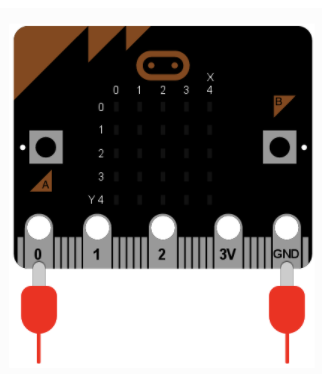
\includegraphics[width=2cm]{1.png}
\caption{microbit配線図}
\label{haisen}
\end{figure}
\subsection{圧電ブザー}
図\ref{haisen}の画像の通りに接続をして、デジタルピンのポート0に1を出力することで音が鳴るよ!\\
\begin{lstlisting} 
from microbit import *
pin0.write_digital(1)
\end{lstlisting}
\subsection{ランダム}
サイコロを作ったね!
\begin{lstlisting} 
from microbit import *
import random
num = ["1", "2", "3", "4", "5", "6" ]
display.scroll(random.choice(num))
\end{lstlisting}
\subsection{スピーカー}
みんなで音楽を作ったね.
図\ref{haisen}の画像の通りに接続をして、デジタルピンのポート0に1を出力することで音が鳴るよ!\\
\begin{lstlisting} 
from microbit import *
import music
notes = ['c4:1', 'e', 'g', 'c5', 'e5', 'g4', 'c5', 'e5', 'c4', 'e', 'g', 'c5', 'e5', 'g4', 'c5', 'e5']
music.play(notes)
\end{lstlisting}
microbitにははじめから曲が用意されているよ!\\
聞いてみよう!
\begin{lstlisting} 
import music
music.play(music.FUNK)
\end{lstlisting}
FUNKを下の曲名に変えてみよう\\
\> \textbf{BIRTHDAY}\\
\> \textbf{DADADADUM}\\
音楽のテンポを設定する関数
\begin{lstlisting} 
music.set_tempo(ticks=4, bpm=120)
\end{lstlisting}
音楽の再生する関数
\begin{lstlisting} 
music.play(music, pin=microbit.pin0, wait=True, loop=False)
\end{lstlisting}
\section{構想}
どんなデスクライトを作ろう?余白を使って構想を練ってみてね!
\end{document}
